
\section{Perception System for Litter Object Localization}
The grapple needs to be able to localize litter objects autonomously underwater, infer the relative position of an object to the grapple, and estimate the litter object metric geometry in preparation for grasping. To this end, we present in the following an overview of the perception system design as shown in Figure~\ref{fig:perception_pipeline}. First, we subscribe to depth and RGB data produced by a passive stereo camera. Secondly, we perform inference with a YOLOv8 object detection deep learning model, trained to detect litter objects underwater. Third, we use the bounding box returned by the object detection inference to create a mask for the depth map produced by the stereo camera, masking the pixel values in the depth mask which don't correspond to the detected object. Fourth, we use the depth map and the masked depth map to construct a voxel map of the scene with static and dynamic elements. Finally, the voxel map, RGB data and object detection model output can be monitored in real-time via Gstreamer and/or Foxglove. The majority of the process, bar the stereo depth estimation computed on-board the stereo camera, is performed on an embedded GPU system, enabling the deployed algorithms to benefit from a high degree of parallelization w.r.t. the computations, ultimately increasing the speed of the pipeline. 

\begin{figure}
    \centering
    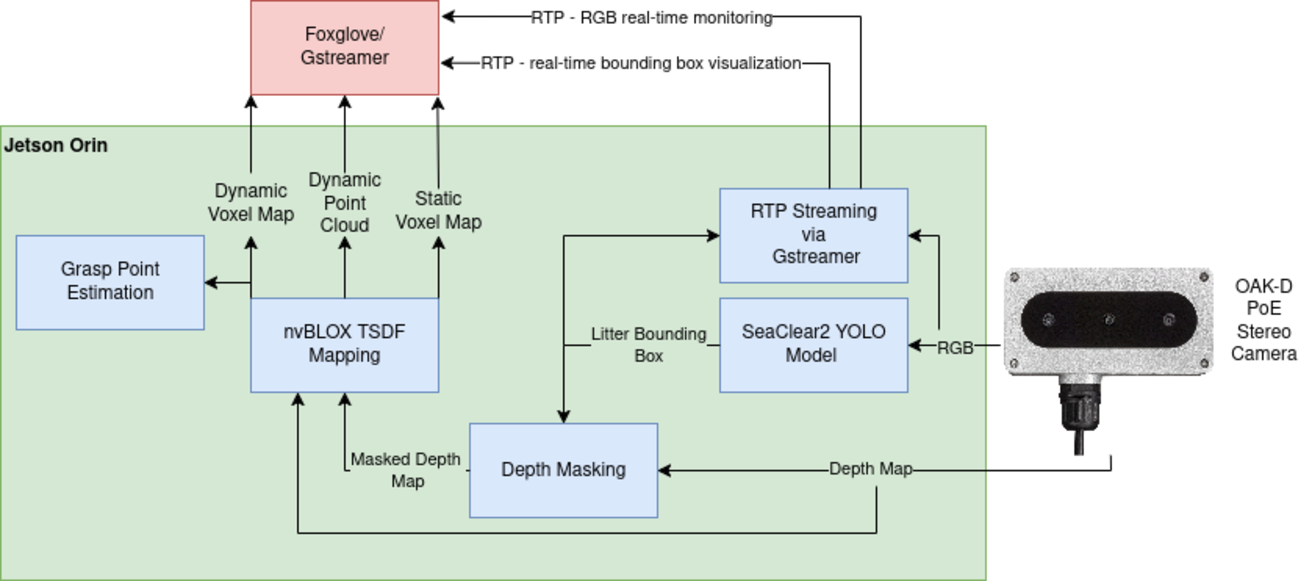
\includegraphics[width=0.9\linewidth]{img/vision_pipeline/vision_system.pdf}
    \caption{An overview of the perception system. The blue boxes represent the processing nodes. The red box the monitoring node(s). The green background indicates the processes that benefit from edge GPU acceleration.}
    \label{fig:perception_pipeline}
\end{figure}

\subsection{Underwater Object Detection}
\label{sec:object_detection}

The SeaClear YOLO based object detection deep learning model for underwater litter objects as described in the Report D4.3, was used as a foundation for the current perception pipeline. The object detection model returns a bounding box around a region in an RGB image at the location of a detected litter object. The bounding box is then 1) laid on top of the actual RGB data and streamed to the surface machine for real-time monitoring, 2) passed to a depth masking node which separates an incoming depth map aligned with the RGB data into "litter object" and "non-litter object" parts. The masked depth mask is then passed to the 3D reconstruction algorithm discussed in Section~\ref{sec:TSDF}.

\subsection{Truncated Signed Distance Function based 3D Reconstruction}
\label{sec:TSDF}

\textbf{Static Voxel Mapping}
\label{sec:static_tsdf}

Compared to point cloud representations, voxel maps approximate each point in 3D space as a voxel, the 3-dimensional equivalent of a pixel. We use the \gls{TSDF}  \bds{For consistency also use the abbreviations latex package in this section} in our approach, which assigns a value corresponding to the (signed) distance of that voxel to the nearest surface. The surface of an object can then be extracted as the location of voxels with distance value 0. This approach provides an estimate for the volumetric properties of objects, informing our grasp planning. 
Additionally occupancy information of the voxels is stored, such as in occupancy grids, where the probability of a voxel being occupied is stored. Each voxel in space is classified as either {\it occupied} or {\it free}, meaning that a particular voxel is either outside of a 3D object if it is {\it free} and situated within the object if it is {\it occupied}.
This dual representation benefits our functionality two-fold. On the one hand the TSDF based voxel map provides a metric estimate of an objects geometry, allowing us to extract volumetric information informing our grasp planning. The occupancy probabilities can be used for obstacle avoidance. \hamish{Described below is the computed 3D reconstruction of objects w.r.t. to the camera frame. In order to relate the spatial and volumetric information of detected objects from the camera frame to the robots frame, we apply a transformation consisting of a rotation and a translation from the camera's base frame to the robot's base frame, defined in the transformation tree of the software stack. This allows the spatial information of objects to be used for planning and visual servoing of the grapple system.}  \bds{how do we convert the objects detected into camera frame into the local map, so that these can be used in the planning or visual servoing phases?} \\
 
Truncated Signed Distance Fields are based on \gls{SDF} which work in the following way. Given a depth map $\mathcal{D}$ , the center point of a voxel w.r.t. the voxel grid coordinate frame $\boldsymbol{p_L}$ and the camera pose w.r.t. the voxel map  $\boldsymbol{T_{CL}}$, we can sample the depth information from the depth map by projecting $\boldsymbol{p_L}$ onto the depth map and assigning the depth value at that point to the corresponding voxel~\cite{Millane2023} 

\begin{equation}
    d = \mathcal{D} \left[ \pi_{camera} \left( \boldsymbol{T}_{CL} \boldsymbol{p_L}  \right) \right]
\end{equation}

where $\mathcal{D} \left[ \boldsymbol{u} \right]$ represents sampling from the depth map at point $\boldsymbol{u}$. The camera projection function $\pi_{camera} \left( \boldsymbol{p_C} \right)$ for a arbitrary point in 3D space $\boldsymbol{p_C}$ is defined as 

\begin{gather}
    \pi_{camera} (\boldsymbol{p}_C) = \frac{1}{ p_{C,z} } 
    \begin{bmatrix}
        f_x& 0& c_x \\
        0& f_y& c_y
    \end{bmatrix}
    \begin{bmatrix}
        p_{C,x} \\ p_{C,y}\\ 1
    \end{bmatrix} 
\end{gather}

where $f_x$, $f_y$, $c_x$ and $c_y$ are the pinhole camera intrinsic parameters which we receive from camera calibration. Now that we have the depth value sampled at the location of the voxel center projected onto the depth map, we subtract the distance of the voxel center to the camera in order to receive the signed distance field value

\begin{equation}
    sdf_i(\boldsymbol{p}_L) = \mathcal{D} \left[ \pi_{camera} \left( \boldsymbol{T}_{CL} \boldsymbol{p_L}  \right) \right] - cam_z( \boldsymbol{p}_L ).
\end{equation}

The result $sdf_i(\boldsymbol{p}_L)$ is the signed distance field value for the voxel. Repeating this procedure for each pixel in-view, i.e. each voxel which can be projected onto the depth map at a given timestep, we can classify each voxel in-view as occupied or unoccupied, extracting the surface of an object as the zero-crossing between occupied and unoccupied values. TSDF is sufficient for surface reconstruction, where all voxel outside of a truncation distance $\epsilon$ are not assigned a value. 

For TSDF, the $sdf_i$ are only considered for voxels within small truncation distance $\epsilon$ away from the surface of objects. The truncated version of the $ sdf_i $ for the $i$-th observation of a scene is defined as $ tsdf_i $ ~\cite{Werner2014}:

\begin{equation}
    tsdf_i(\boldsymbol{p}_L) = \max\left(-1,   \min \left( 1 , \frac{sdf_i(\boldsymbol{p}_L)}{ \epsilon} \right) \right)
\end{equation}

\begin{figure}
    \centering
    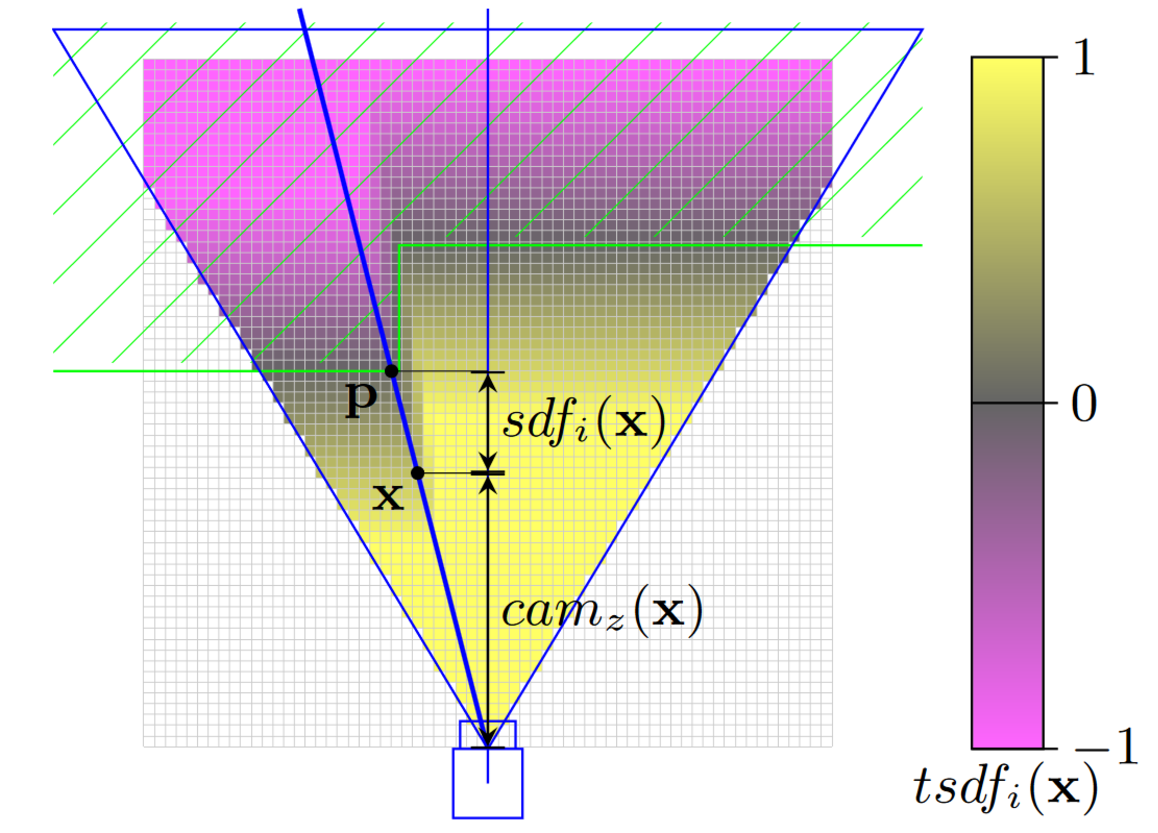
\includegraphics[width=0.5\linewidth]{img/vision_pipeline/tsdf_illustration.pdf}
    \caption{The 3D object in space is denoted in green. The truncated distance values are denoted in color from pink to yellow. In this case an exemplary truncation distance $ \epsilon $ is set to $1$~\cite{Werner2014}.}
    \label{fig:sdf_illustration}
\end{figure}

An illustration of how signed distance fields work can be seen in Figure \ref{fig:sdf_illustration}, here computing the distance of voxel $\boldsymbol{x}$ to the surface point $\boldsymbol{p}$ is illustrated. The colored regions in Figure \ref{fig:sdf_illustration} indicate the values within the truncation threshold.

Voxel grids can be efficiently implemented for GPU acceleration. The grid is divided into larger  chunks of voxels, e.g. an 8x8x8 block, and each chunk is stored within GPU memory; each block is then continuously updated in parallel by the GPU, freeing up voxels that are no longer occupied, assigning depth values to newly observed voxels and updating distances as the camera moves through the scene.

\newpage

\textbf{Dynamic Voxel Mapping}
\label{sec:dynamic_tsdf}

\begin{figure}[!htbp]
    \centering
    \begin{minipage}{0.4\textwidth}
        \centering
        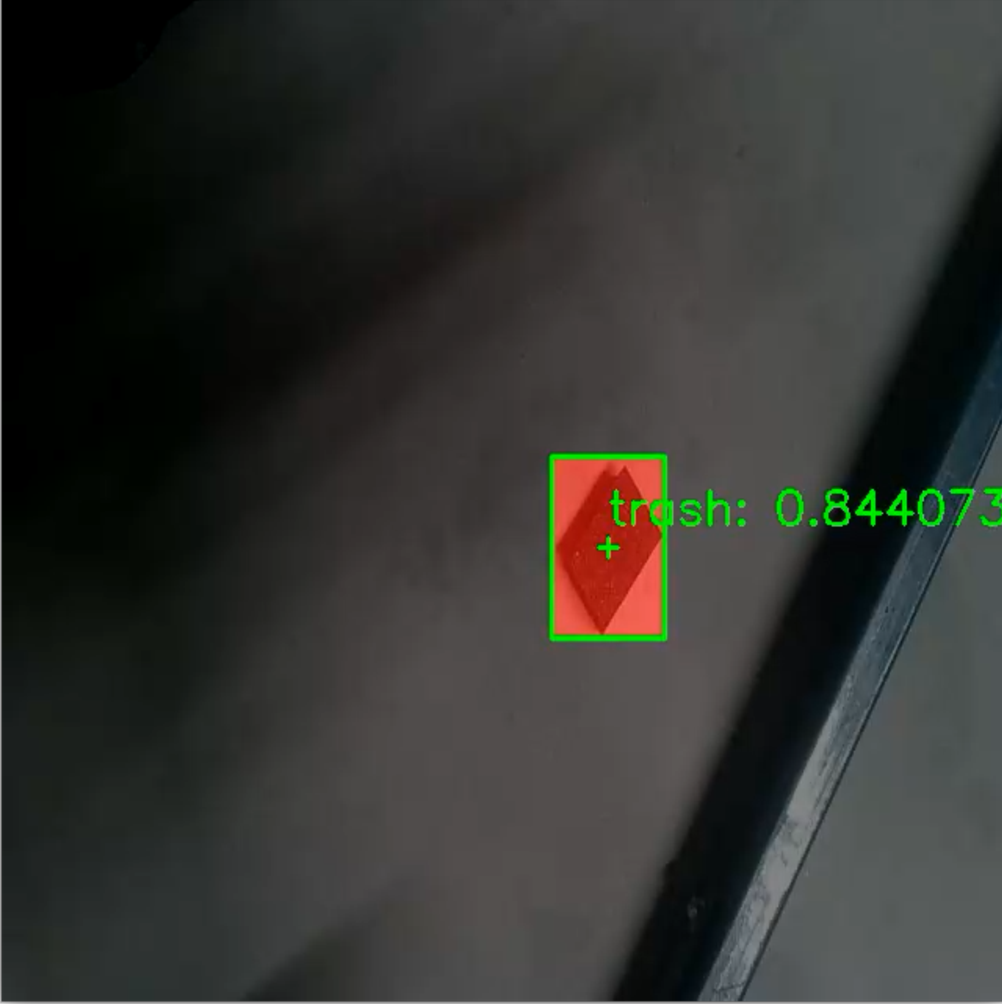
\includegraphics[width=\linewidth]{img/vision_pipeline/detection_in_air.pdf}
        \caption{The bounding box returned by the object detection model post-processed and laid on top of the RGB data from the downward facing stereo camera. }
        \label{fig:object_detection}
    \end{minipage}\hfill% <-- Keep this comment here!
    \begin{minipage}{0.4\textwidth}
        \centering
        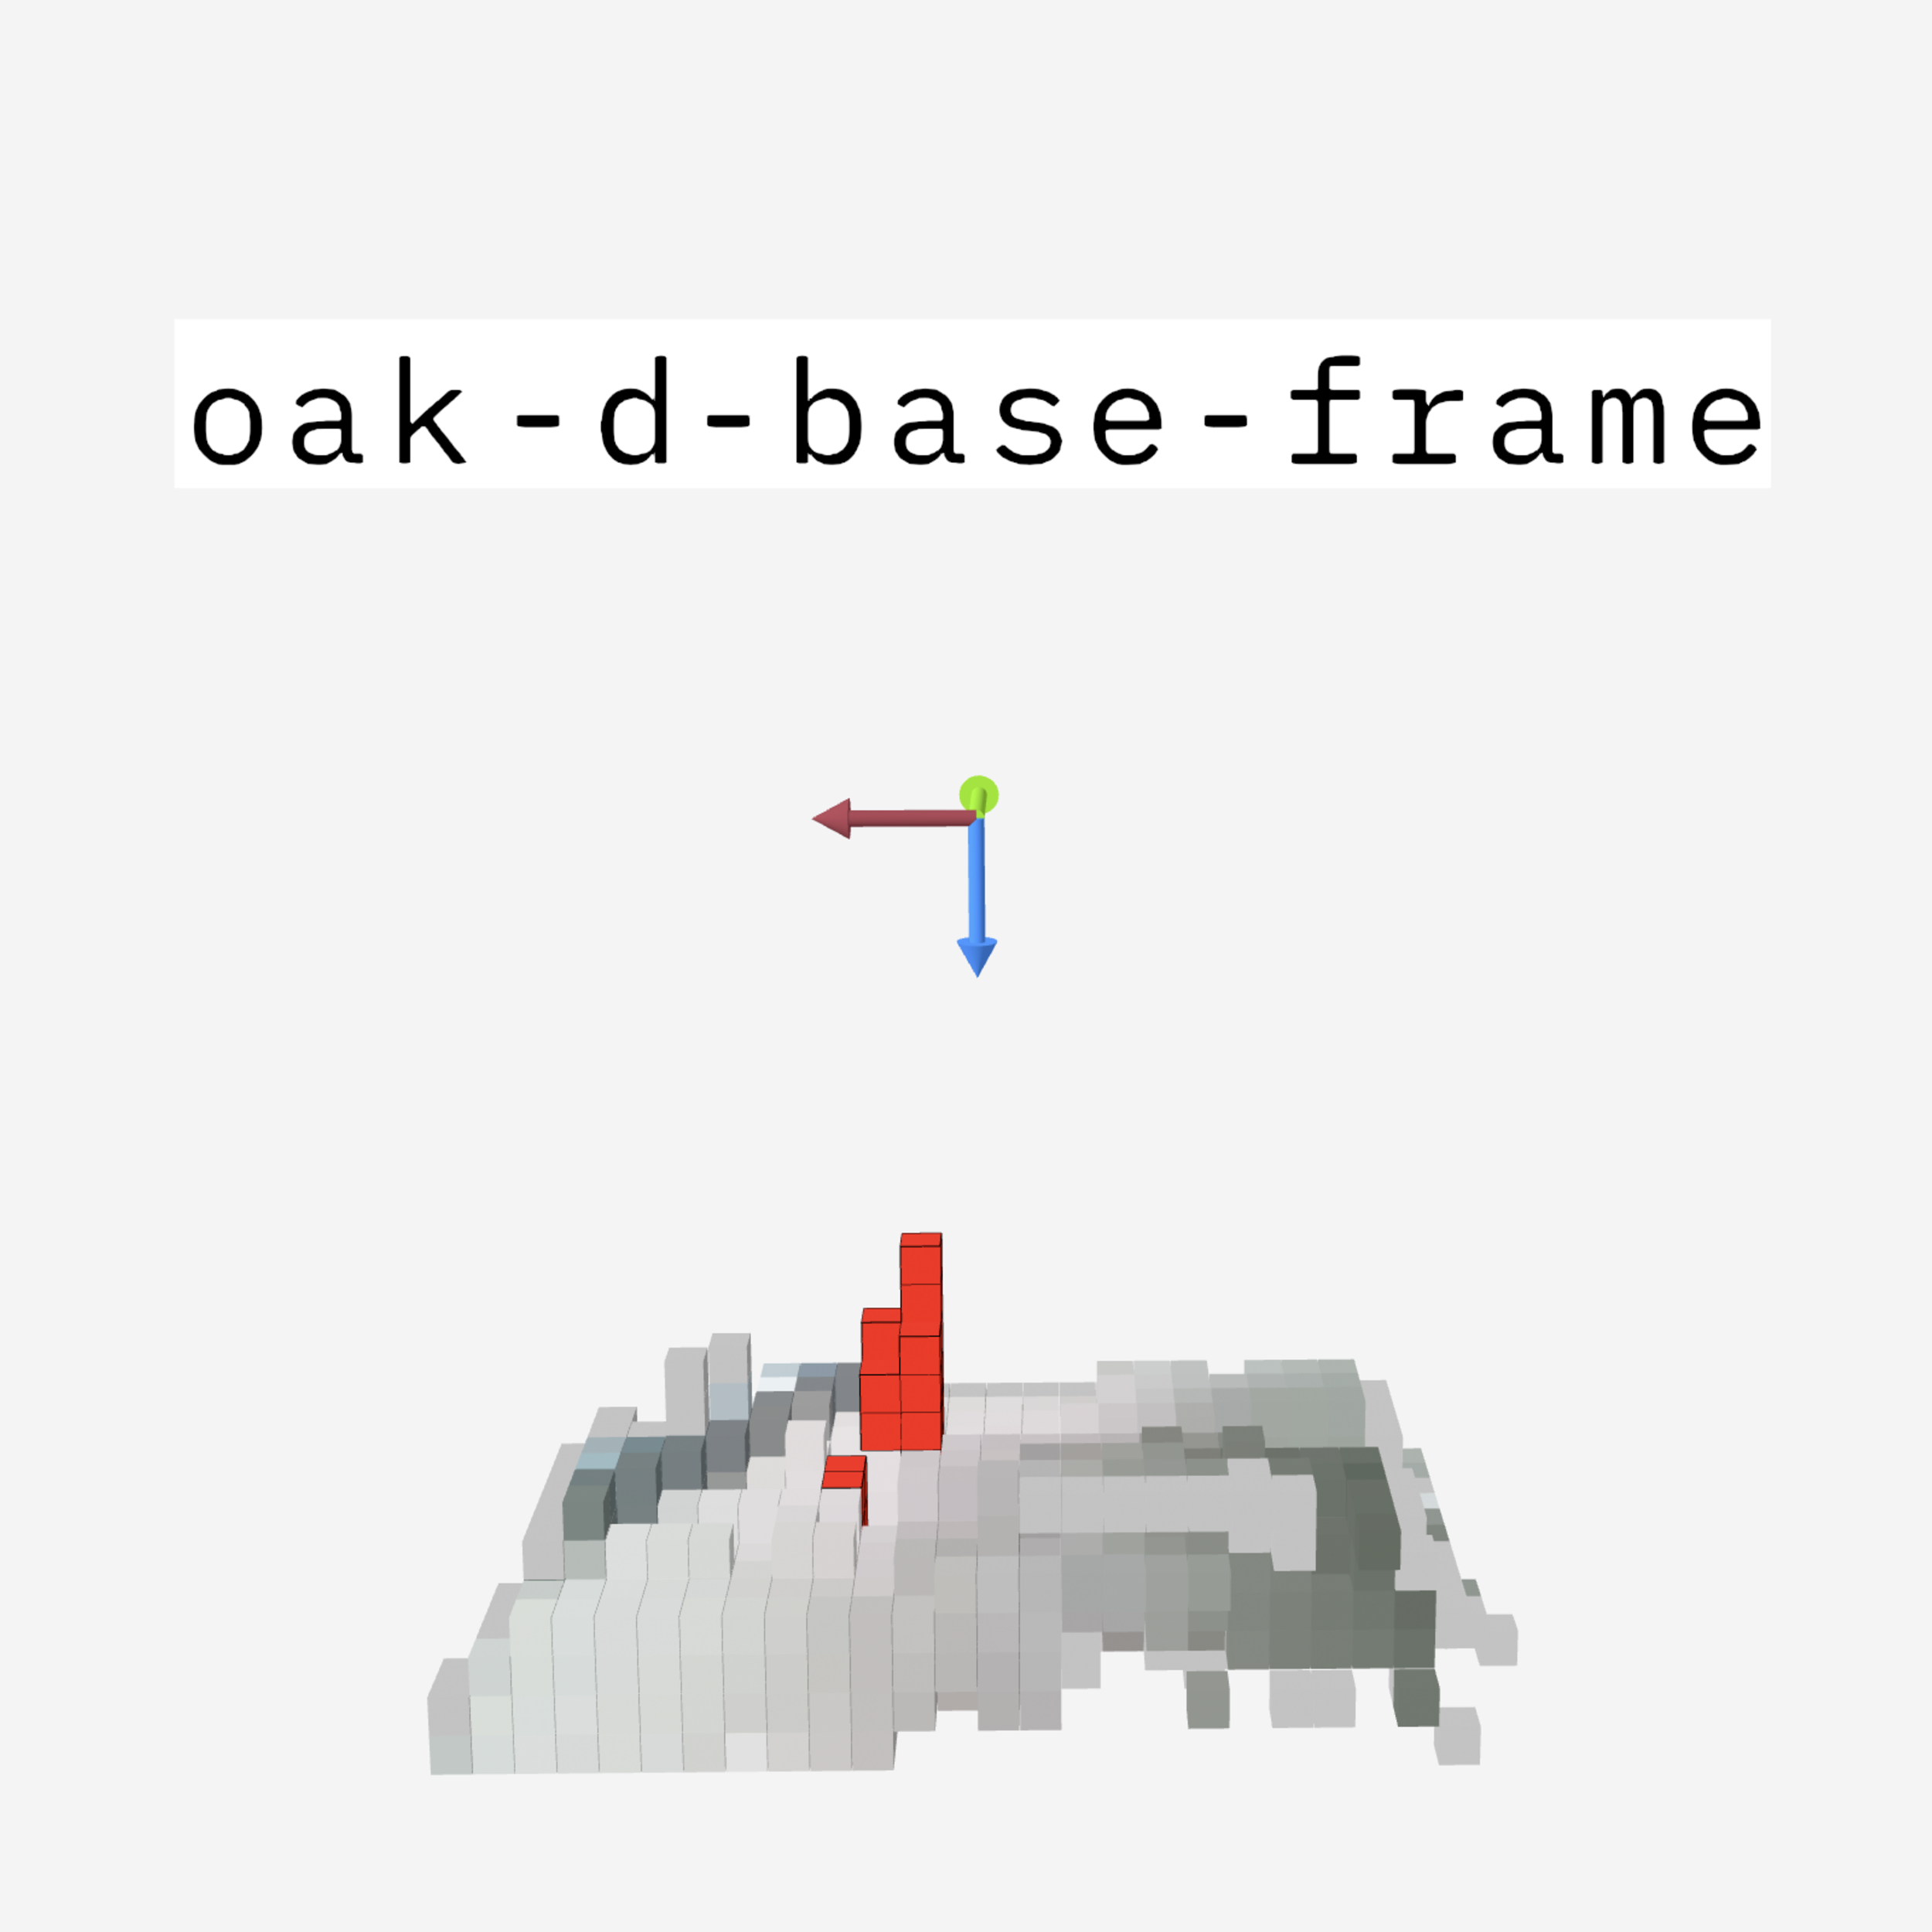
\includegraphics[width=\linewidth]{img/vision_pipeline/tsdf_in_air.pdf}
        \caption{The static and dynamic voxel layers computed from the input scene in Figure \ref{fig:object_detection}. The red voxels correspond to the litter object detected by the model.}
        \label{fig:image2}
    \end{minipage}
    \label{fig:object_detection_tsdf}
\end{figure}

So far we have only discussed mapping of a static scene by the \gls{TSDF} algorithm. Mapping the whole scene is computationally expensive even in the \gls{TSDF} case. Since we receive a bounding from from the object detection model, we use this to reduce the region of interest for applying \gls{TSDF}. The bounding box received from the object detection applied to the RGB data as discussed in Section~\ref{sec:object_detection}, is used to mask the depth map from the stereo camera into litter object parts and non-litter object parts. The voxel map is then separated into a static and a dynamic layer, where the static layer is computed as before, but the dynamic layer now only contains voxels computed from the masked depth values, i.e. contains voxels that correspond to a detected object. We can then apply grasp point estimation to the dynamic layer corresponding to the detected object. 

We relax the assumption that only static objects are reconstructed by the algorithm from Section~\ref{sec:static_tsdf}, since this allows the bounding box to move within the scene if e.g. the object is moved by ocean dynamics. For this, we need to apply a decay step to the occupancy values of the voxels. At a fixed frequency, all voxel occupancy probabilities are decayed towards 0.5 over time. This means that the state of a voxel (occupied or free) becomes less certain after it has fallen out of view until it becomes unknown i.e. the voxel holds 0.5 occupancy probability. 

